\chapter{Discussion}

\subsection{Confusion Network}

It is natural to mix up the places that are geographically very close, have similar names or seem somehow similar for entirely different reasons. For example, students typically know the approximate geographical location of the Nordic countries, however they might struggle when determining its exact location, often they confuse Norway with Sweden as can be seen in Figure~\ref{fig:confusion-network}. If a students chooses Finland when the highlighted place is actually Norway, it usually doesn't mean that they have no knowledge of the country's location. In such cases it seems reasonable to perhaps slightly increase student's knowledge of the place.

\begin{figure}[htbp]
  \centering
  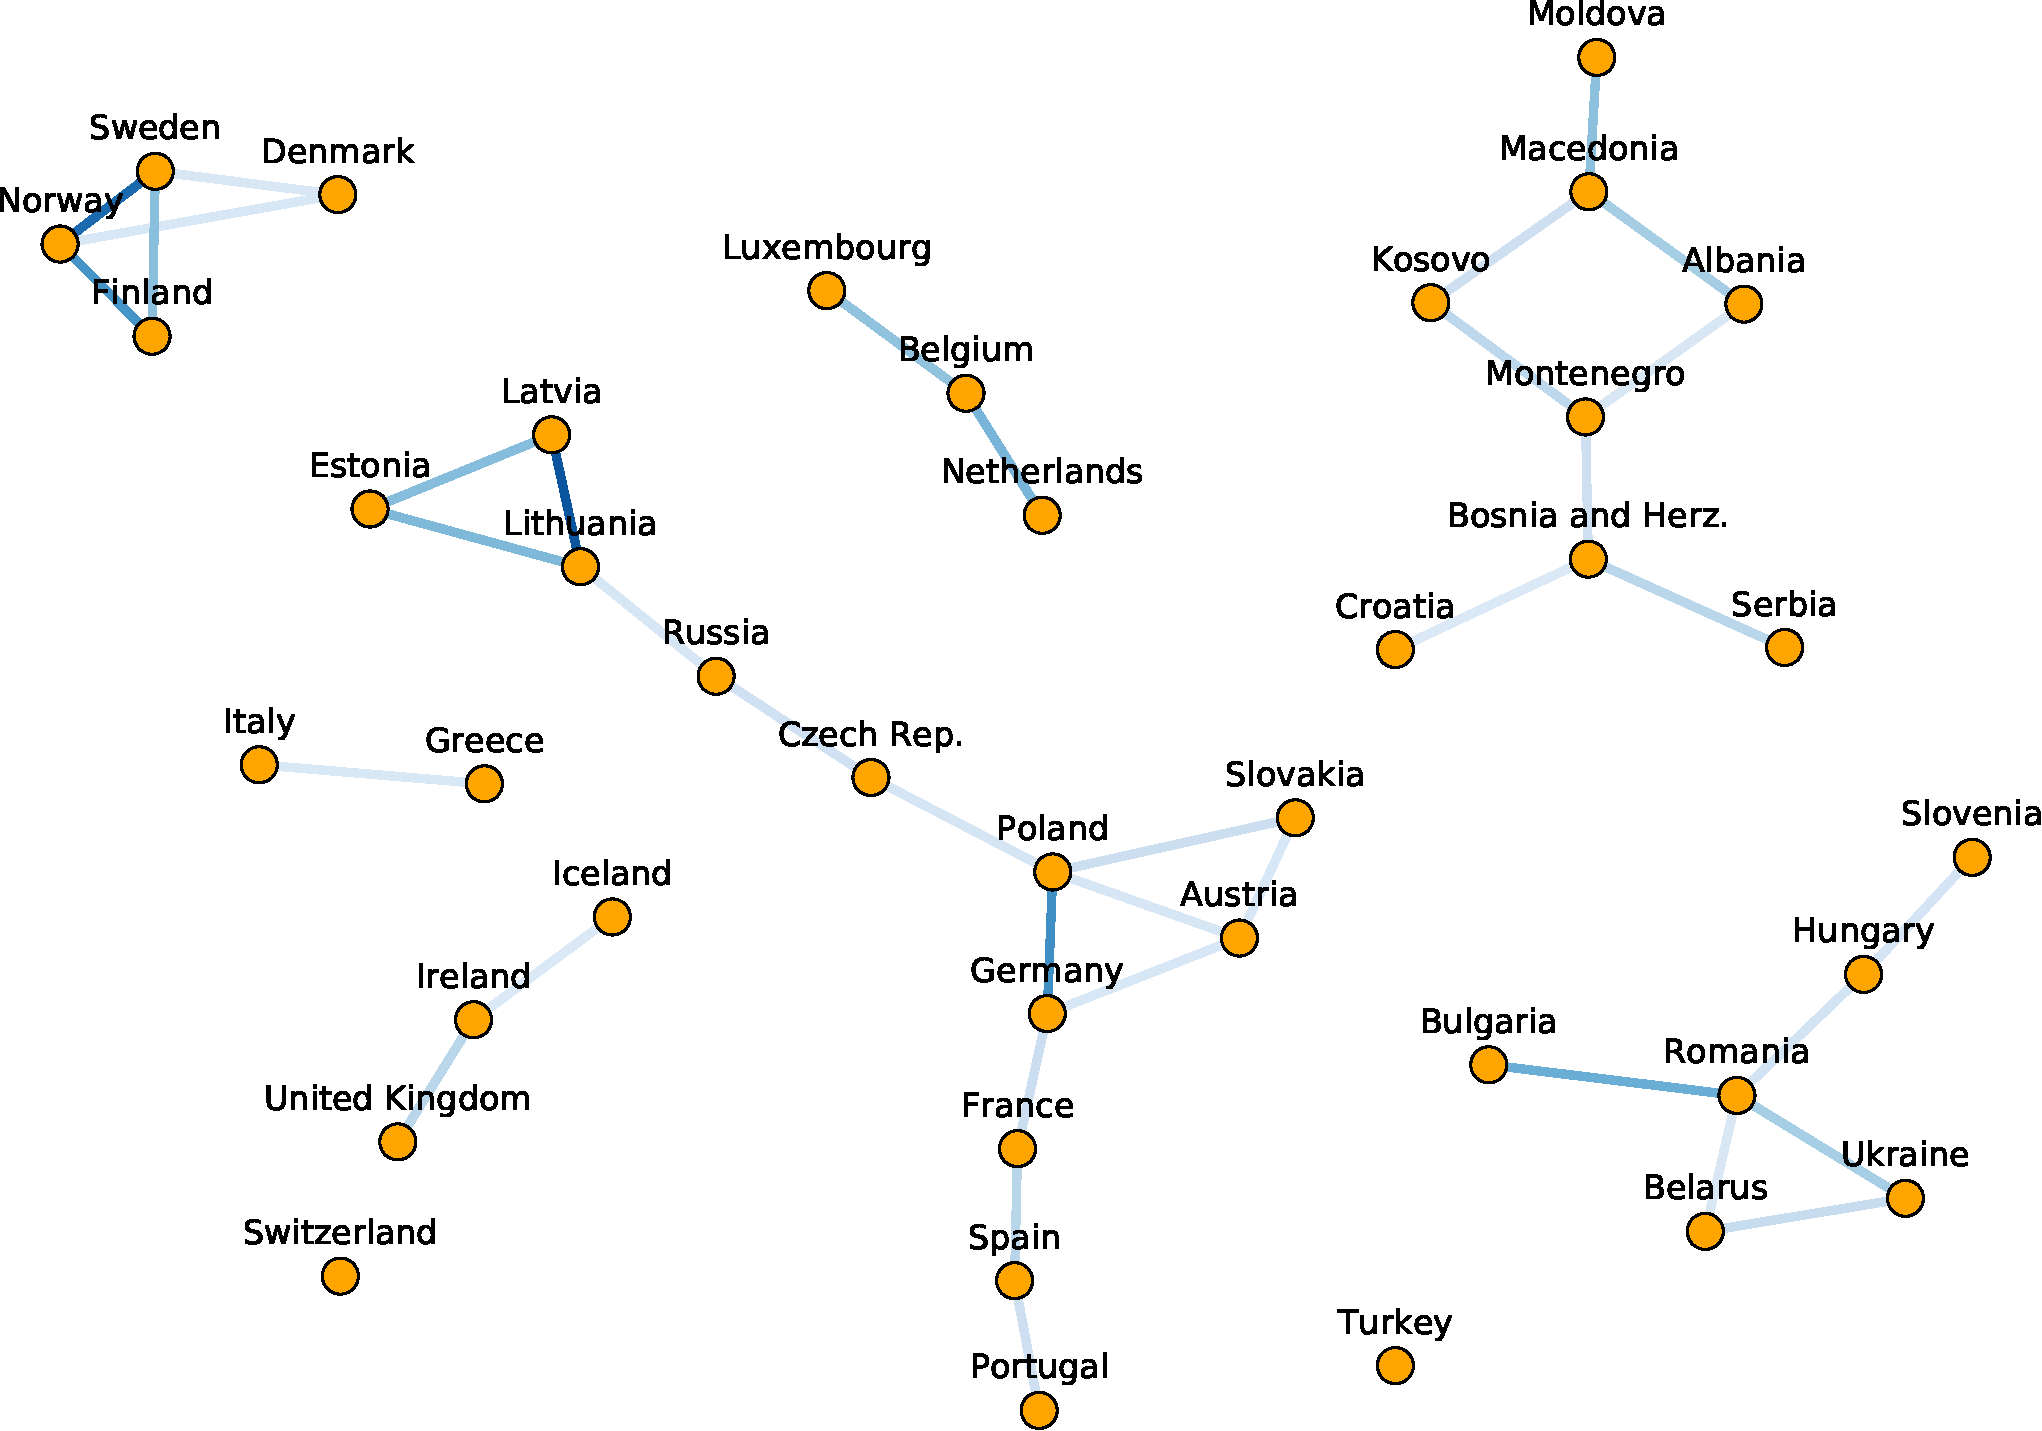
\includegraphics[width=\textwidth]{img/confusion-network}
  \caption{Confusion network of European countries. The edges between countries represent confusion of students. Dark blue edge means that the two connected countries are confused by students quite often while light blue indicates that the countries are still sometimes confused but at least less often.}
  \label{fig:confusion-network}
\end{figure}
